\documentclass[11pt]{article}
\usepackage{cite}
\usepackage{fancyhdr}
\usepackage[svgnames]{xcolor}
\usepackage{url}
\usepackage{tikz}
\usetikzlibrary{shapes,snakes,arrows}
\usepackage{hyperref}

\topmargin=-5mm
\evensidemargin=0cm
\oddsidemargin=0cm
\textwidth=16cm
\textheight=22cm
\addtolength{\headheight}{1.6pt}
\hypersetup{pdfstartview=}

\tikzset{>=latex}

\newcommand{\secref}[1]{\S\ref{#1}}

\newcommand{\lastupdate}{\today}
\newcommand{\ie}{\textit{i.e.}}
\newcommand{\mdash}{---}
\newcommand{\ecall}{\textsf{ecall}}
\newcommand{\ocall}{\textsf{ocall}}
\newcommand{\env}{\textsf{environment}}
\newcommand{\mrenclave}{\textsf{mrenclave}}
\newcommand{\mrsigner}{\textsf{mrsigner}}
\newcommand{\sha}{\textsf{sha256}}
\newcommand{\pve}{\textsf{PvE}}
\newcommand{\pce}{\textsf{PcE}}
\newcommand{\qe}{\textsf{QE}}

% \lhead{\sc On the insufficiency of Intel SGX Remote Attestation}
% \rhead{\sc \lastupdate}

\title{\bf A Framework for analyzing Intel SGX Enclaves}
\author{\textsc{Yogesh Prem Swami}}

\date{\lastupdate}

\begin{document}
\pagenumbering{arabic}

\maketitle

\begin{abstract}
  Intel SGX enclaves  provide hardware
  enforced confidentiality and integrity guarantees for running pure
  computations (\ie, OS-level side-effect-free code) in the cloud
  environment. In addition, SGX remote attestation enables
  enclaves to prove that a claimed enclave is indeed running inside a
  genuine SGX hardware and not some (adversary controlled) SGX
  simulator.

  Since cryptographic protocols do not compose well
  \cite{ucframework} especially when run concurrently, SGX remote
  attestation is only a necessary pre-condition for securely
  instantiating an enclave. In practice, one needs to analyze all the
  different interacting enclaves as a single protocol and make sure
  that no sub-computation of the protocol can be simulated outside of
  the enclave. In this paper, we present a practical framework for
  analyzing enclaves. We analyze Intel provided EPID\cite{epid}
  \textsf{Provisioning} and \textsf{Quoting} Enclave\cite{sgxattest}
  within this framework and report our (largely positive) findings. We
  also provide details about SGX's use of EPID and report
  (largely negative) results about claimed anonymity guarantees.
\end{abstract}

\section{Introduction}
  Intel SGX enclaves\cite{sgxinnov, sgxinnov2} provide hardware
  enforced confidentiality and  integrity guarantees for running pure
  computation (\textit{i.e.}, OS-level side-effect-free code) in the
  cloud environment. By limiting the application's Trusted Computing
  Base (TCB) to the CPU and CPU-Cache, SGX provides unprecidented
  confidentiality and integrity guarantees against malicious OS
  kernels and supervisor software. Since a remote user cannot be sure
  if an enclave is indeed running on a real-hardware instead of a
  software simulator (such as QEMU), SGX provides a remote attestation
  mechanism to prove to third parties that an enclave has indeed been
  instantiated on a real hardware.

  Given such strong guarantees, a popular design methodology for
  creating secure cloud applications is to:

  \begin{itemize}
    \item Compose multiple independent well-known protocols inside the
      enclave to create a larger protocol, and

    \item Depend on remote attestation to ensure that different parts
      of the protocol can only
  \end{itemize}

  Good examples of this methodology are \cite{Haven, Graphene, Scone},
  where the authors try to run unmodified (or minimally modified)
  applications inside the enclave, and depend upon remote-attestation
  to make sure that the internal state of the application will not be
  compromise.

  \section{SGX Computational Model}
  \label{sec:model}
  Intel documentation\cite{intelsdm} provides excellent low-level
  details about the SGX instructions. This section provides an
  abstract computational model of SGX which is better suited for
  security analysis of an SGX enclave.

  Abstractly, an SGX enclave can be thought of as a blackbox that's
  capable of running any arbitrary algorthim. The blackbox, hereafter
  called an enclave, communicates with the outside world, called the
  \env, in three different ways:

  \begin{figure}[h]
  \centering
  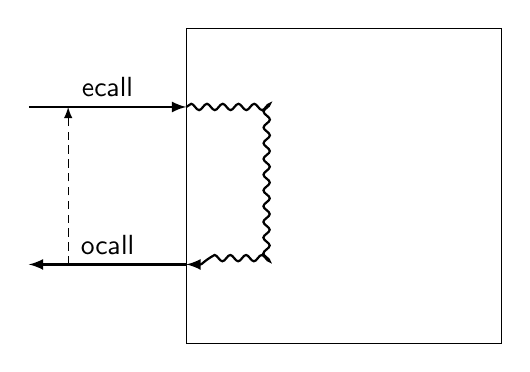
\begin{tikzpicture}[x=1cm, y=-1cm]
  \newcommand{\ench}{4cm}
  \newcommand{\encw}{4cm}
  \newcommand{\alen}{1cm}
  \newcommand{\adiff}{1cm}

  \node[rectangle, minimum height=\ench, minimum width=\encw, draw] (enc) {};
  \draw[->,thick] (-\encw / 2.0 - 2*\alen, \adiff ) -- (-\encw/2.0, \adiff) %%
  node [midway, above] {\textsf{ecall}};

  \draw [->, thick, decorate, %%
    decoration={snake,amplitude=.4mm,segment length=2mm, post length=1mm}] %%
  (-\encw/2.0, \adiff) -- (-\encw/2.0 + 1*\adiff + 0.1, \adiff) -- %%
  (-\encw/2.0 + 1*\adiff , -\adiff) -- (-\encw/2.0, -\adiff);


  \draw[<-,thick] (-\encw / 2.0 - 2*\alen, -\adiff ) -- (-\encw/2.0, -\adiff) %%
  node [midway, above] {\textsf{ocall}};

  \draw[->, thin,densely dashed] (-\encw / 2.0 - 1.5*\alen, -\adiff ) -- %%
  (-\encw/2.0 - 1.5*\alen , \adiff);
\end{tikzpicture}

  \caption{SGX Computational Model.}
  \label{fig:model}
  \end{figure}

  \begin{description}
  \item[Ecall]: The \env\ can invoke a pre-defined function inside the
    enclave by passing input parameters and returning internal state
    of the enclave as results. Such invocations from the \env\ to the
    enclave are referred to as \ecall. The parameter values passed
    from the \env\ to the enclave are either copied or directly shared
    with the enclave. An \ecall\ can terminate in one of the three
    ways: (a) by returning from the enclave, (b) by making an explicit
    \ocall, or (c) as a result of an interrupt or exception.

    SGX also supports multithreading, and it's possible for the
    \env\ to run the same \ecall\ in different threads. However, once
    an \ecall\ has acquired the thread, future attempts to reuse that
    same thread will result in error. Futhermore, the number of
    threads that an enclave can support is pre-determined by the
    enclave signer, and cannot be altered at runtime.

  \item [Ocall]: While an enclave is executing (because of some
    previous \ecall), it can make \ocall s  to pre-designated
    functions in the \env.  Unlike an \ecall, an \ocall\ cannot
    directly share the internal enclave state with the \env, and
    must---directly or indirectly---copy the parameters into the
    \env\ before making an \ocall.

    An interesting characteristic of an \ocall\ is that the \env\ is
    not requred to return back to the enclave at the end of the
    \ocall\ (see \ref{fig:model}). Since the behavior of pre-designated
    functions in the \env\ are controlled by the adversary, one should
    not expect the \env\ to follow the protocol that enclave author
    envisioned. In particular, it's possible to create a chain of
    \ecall s and \ocall s such that the adversary can perform
    operations on the internal (global) state of the enclave.

  \item[Asynchrnonous Exit] In addition to an \ocall, the
    processor can exit from an enclave due to an interrupt or
    exception. Such enclave exiting events are called Asynchronous
    Exit Events, or AEX. Unlike an \ocall, an AEX can transfer control
    from the enlave to the environment at arbitrary (possibly adversary
    controlled) points inside the enclave. Like \ocall s, an AEX can
    either by resumed from where the enclave left off, or the
    environment can invoke another \ecall (either within the same
    thread or a different thread).

    Since an adversary can create multiple running copies of an
    enclave and selectively interrupt each enclave to cause and AEX,
    it can be used as a means to ``rewind'' the internal state of of
    the enclave. Given that proof-of-knowledge \cite{BellarePOK}
    protocols fundamentally have a \textit{knowledge-extractor} based
    on rewinding, an enclave must ensure that it does not leak secrets
    when interrupted by an AEX.

  \end{description}

  \subsection{Enclave Creation}
  \label{sec:enclavecreateion}
  An enclave is generated as a dynamically shared library using
  standard compiler tools. In addition, the entity creating the
  enclave must also decide up-front on the following information:

  \begin{description}
    \item[Attributes]: The attributes of an enclave act as an access
      control mechanism that is enforced by the hardware. For example,
      certain high priviledge keys, such as Launch-Key and Provision-Key 
      cannot be made accessible to all the enclaves, as it would 
      compromize the security of entire SGX ecosystem---not just a 
      given CPU. An enclave author requests the attributes needed by 
      the enclave at compiler/sign time, and the Launch-Enclave, based 
      on policy decisions, decides whether to grant or reject an 
      authorization token (called \textsf{EINITTOKEN}) for instantiating 
      the enclave.
    \item[Stack size]: The enclave author must estimate the size of the
      stack needed by enclave and set its value at enclave creation time. 
      Once an enclave is instantiated, this value cannot be changed.

    \item[Heap size]: Like the stack size, the heap-size of the enclave 
      is also fixed at enclave creation time. In SGXv2, this value can 
      be changed post instantiation.

    \item[Thread count]: An enclave must also decide upon the number
      of threads that can run conconrrently. As pointed out in
      \secref{sec:model}, concurrency can have a dramatically negative
      impact on the security of the certain protocols, and one must
      not select this parameter just on the basis of performance 
      requirements, but also on the basis of security concerns.
    
    \item[Software versioning]: SGX provides elaborate software-upgrade 
      and life-cycle management faciliaties and allows software vendors 
      to make use of these features.

  \end{description}
  Based on these parameters, the enclave signing tool creates a
  virtual memory layout of the enclave and comptes a hash of the
  entire memory layout (including the stack, heap, thread control
  structure, etc.)  See \cite{intelsdm} for details
  about how the hash is computed. This hash, called
  \mrenclave, is used as the unique identifier for the enclave.

  In addition to \textsf{mrenclave}, the software vendor must
  also sign the enclave using a RSA-3072 key. The hash of the RSA
  Public-Key is called \mrsigner. As described in \cite{surnaming},
  the purpose of the signature is to provide an unforgeable
  identity---a \textit{surname} based lineage---to a set of enclaves
  based on the vendor.

  It should be noted that the \mrenclave\ of an enclave doesn't
  change even when the signing key is changed. This is significant
  when validating attestation or deriving keys based on
  \mrenclave.

  \subsection{Enclave Instantiation and Access Control}
  An properly signed enclave can run on any Intel SGX
  Processor. However, before an enclave can be instantiated, it must
  get an authorization token, called \textit{Launch Token}, from Intel
  provided \textsf{Launch Enclave}. The \textsf{Launch Enclave}
  enforces policies either on the basis of \mrenclave, \mrsigner, or
  the attributes of the enclave (such as, whether the enclave is in
  debug mode) or based on an Intel signed whitelist. (Since SGX
  doesn't have any in-built mechanism for replay protection, once
  Intel adds an enclave to the whitelist, it can practically never be
  removed.)

  \subsection{SGX Platform Keys}
  \label
  As described in \cite{sgxattest}, each Intel SGX capable processor
  contains two statistically independent base keys:
  \textit{Root Provisioning Key} and \textit{Root Seal Key}. The Root
  Provisioning Key is used as the Root of trust between the CPU and
  Intel Attestation Services (IAS) \cite{ias}. Intel retains a copy
  of this key at the time of manufacturing and uses it to establish
  the trustworthiness of the processor during EPID join process. Intel
  claims that \textit{Root Seal Key} is not retained. However, it's
  not clear whether the this key is generated inside the processor via
  oracle access (\ie, in such a way that CPU generates the key all by
  itself using it's own internal random numbers or with PUFs), or
  whether the key is first generated outside the processor, then
  injected into CPU, and finally destroyed. Unless the keys are
  generated via oracle access (and Intel can provide a proof to 
  this effect), one should consider the Root Seal Key to be 
  known to Intel.

  An application software does not have raw acceess to these base 
  keys. However, an application can access several \textit{named} 
  keys that derived from the base key:

  \begin{description} 
    \item[Provisioning Key]: This key is derived from Root
      Provisioning Key and is used as the root-of-trust 
      between the CPU and the Intel Attestation Service during the 
      EPID join process. Since admitting a non-SGX processor to 
      the Intel Attesttion Service's group of SGX Processors will 
      completely compromize Remote Attestation of all CPUs, extreme 
      care must be taken in granting access to Provisioning Key. 
      Currently, the Launch Enclave only grants Provisioning Key 
      access to enclaves that have been signed by Intel. Furthermore,
      only Provisioning Enclave (\pve) and Provisioning Certification 
      Enclave (\pce) (both created without debug option) have access to 
      Provisioning Key.

    \item[Provisioning Seal Key]: This key is derived joinly from Root
      Provisioning Key and Root Seal Key. The EPID join process, the 
      EPID private-key for each platform is encrypted with this key
      and uploaded to Intel Attestation Service. (See \secref{ssec:epidprov}
      for details about EPID Join process.)

      Note that the EPID private-key could not just be encrypted with
      Provisioning Key as that would destory the EPID's blinded-join 
      protocol. Conversely, the EPID private-key cannot be encrypted
      just with Seal Key as that might allow non-priviledged enclaves
      to have access to EPID private key and thereby render Remote 
      Attestation ineffective\footnote{If someone can access EPID 
      private key, they can sign remote attestation queries for 
      \textit{any} platform. Furthermore, because of unlinkability, 
      it will be impossible to determine which platform was abused.}. 

      In spite of this design choice, given the uncertainity about 
      how the Root Seal Key is generated, one should assume that 
      Intel knows the EPID private key for each platform.

      \item[Launch Key]: This key is derived from Root Seal Key and 
      is used by Launch Enclave to create authorization tokens 
      (\textsf{EINITTOKEN}) that each non-Intel enclave must obtain 
      in order to instantiate an enclave. Currently, only a specific 
      \mrsigner---whose corresponding private-keys are only known 
      to Intel---can access this Key. In SGXv2, the \mrsigner for 
      Launch Key can be changed programatically, and any enclave 
      signed with that \mrsigner can gain access. With this change, 
      however, it's not clear how Intel intends to protect the 
      Proviosioning Key.

      \item[Seal Key]: This key is derived from Root Seal Key and used
      for encrypting data specifically for a given CPU.

      \item[Report Key]: This key is derived from Root Seal Key and used 
      for generating Local Attestation report \secref{sec:localatt}.

  \end{description}

  \subsection{SGX Platform Enclaves}
  

  \section{Framework for Analyzing SGX Enclave}
  \subsection{Concurrent Enclave Execution}
  \subsection{Parallel Enclave Execution}
  \subsection{Enclave Rewinding}

  \section{Local Attestation}
  \label{sec:localatt}

  \section{SGX Remote Attestation}
  \label{sec:remoteatt}

  \subsection{EPID Overview}
  \label{ssec:epid}

  \subsection{SGX Pairing Groups}
  \label{ssec:pairings}

  \subsection{SGX EPID provisioning}
  \label{ssec:epidprov}
  
  \subsection{SGX Quoting Enclave}
  \label{ssec:qe}

  \section{Conclusion}
  \label{sec:conclusion}

\bibliographystyle{alpha}
\bibliography{sgx_biblio}

\end{document}
